
\begin{frame}{Sharing of code \& data mandatory in many journals}

  
  \begin{figure}
    \centering
    \includegraphics<1>[width=0.95\textwidth]{%
      img/science_policy.png} %
    \includegraphics<2>[width=0.95\textwidth]{%
      img/science_policy_t1.png} %
    \includegraphics<3>[width=0.95\textwidth]{%
      img/science_policy_t2.png} %
  \end{figure}

  \vspace{0.4cm}
  
  \begin{flushright}
    \small Policy of \textit{Science} since February 11, 2011
  \end{flushright}

  \pnote{
    
    Now that we established computational reproducibility\\
    should be simple and journals are demanding\\
    sharing anyway, we're good, right?

    How effect is such an policy?
    
  }
  
\end{frame}

\begin{frame}{}
  
  \begin{figure}
    \centering
    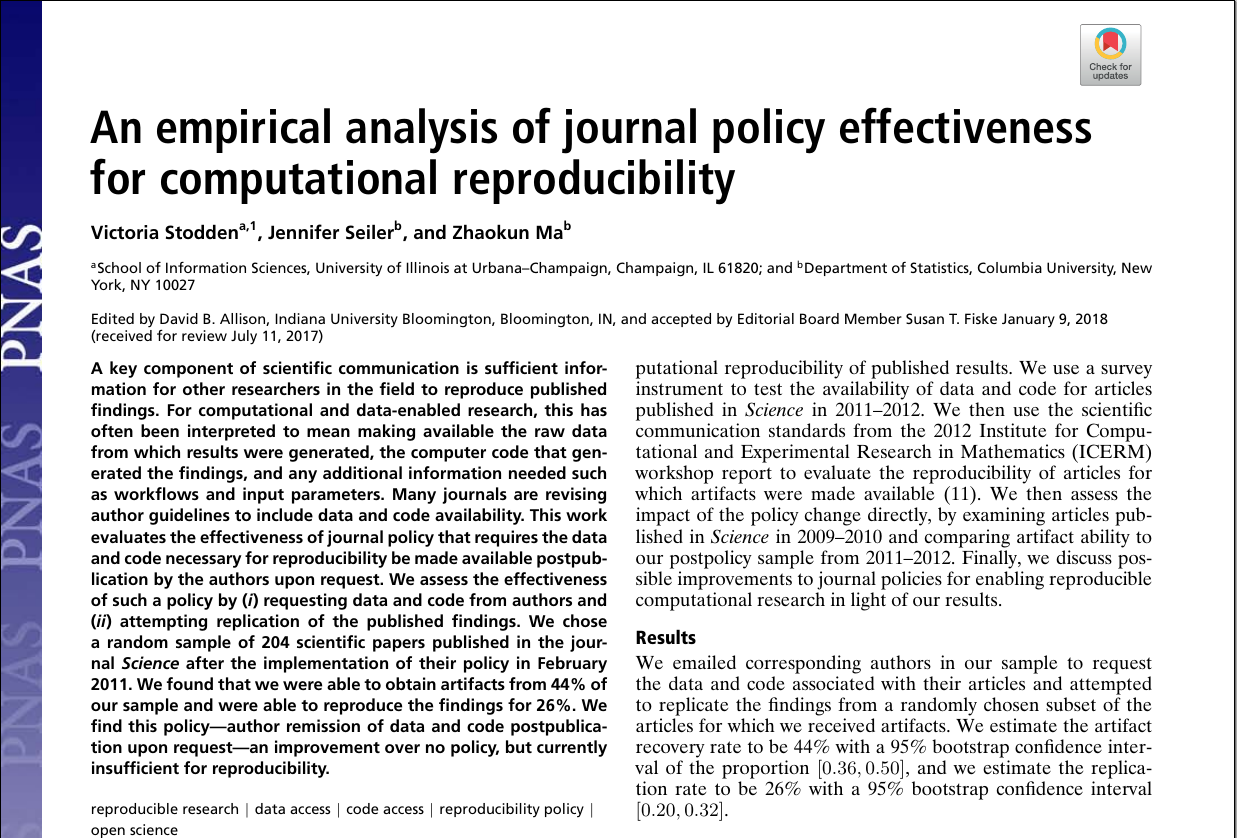
\includegraphics[width=0.875\textwidth]{%
      img/stodden2018_cover3.png} %
  \end{figure}
  
  \vspace{0.015cm}

  \begin{center}
    Out of 206 computational studies in \textit{Science} since 2011, \\
    26 provided code \& data directly  
  \end{center}
  

  \source{\cite{Stodden2018}}

  \pnote{
    
    To the remaining 180 studies \\
    the authors sent Emails asking \\
    for the code for the studies
    
  }

  
\end{frame}


\begin{frame}{A few responses...}
  
  \begin{figure}
    \centering
    \includegraphics<1>[width=0.95\textwidth]{%
      img/stodden2018_re1.png} %
    \includegraphics<2->[width=0.95\textwidth]{%
      img/stodden2018_re1_op.png} %

  \end{figure}

  \begin{figure}
    \centering
    \includegraphics<1>[width=0.95\textwidth]{%
      img/stodden2018_re2_op.png} %
    \includegraphics<2>[width=0.95\textwidth]{%
      img/stodden2018_re2.png} %
    \includegraphics<3>[width=0.95\textwidth]{%
      img/stodden2018_re2_op.png} %

  \end{figure}

  \begin{figure}
    \centering
    \includegraphics<1-2>[width=0.95\textwidth]{%
      img/stodden2018_re3_op.png} %
    \includegraphics<3>[width=0.95\textwidth]{%
      img/stodden2018_re3.png} %
  \end{figure}

  \source{\cite{Stodden2018}}
  
\end{frame}



\begin{frame}{\large   Of $N=206$ articles published in \textit{Science} since 2011...}


  \begin{figure}
    \centering
    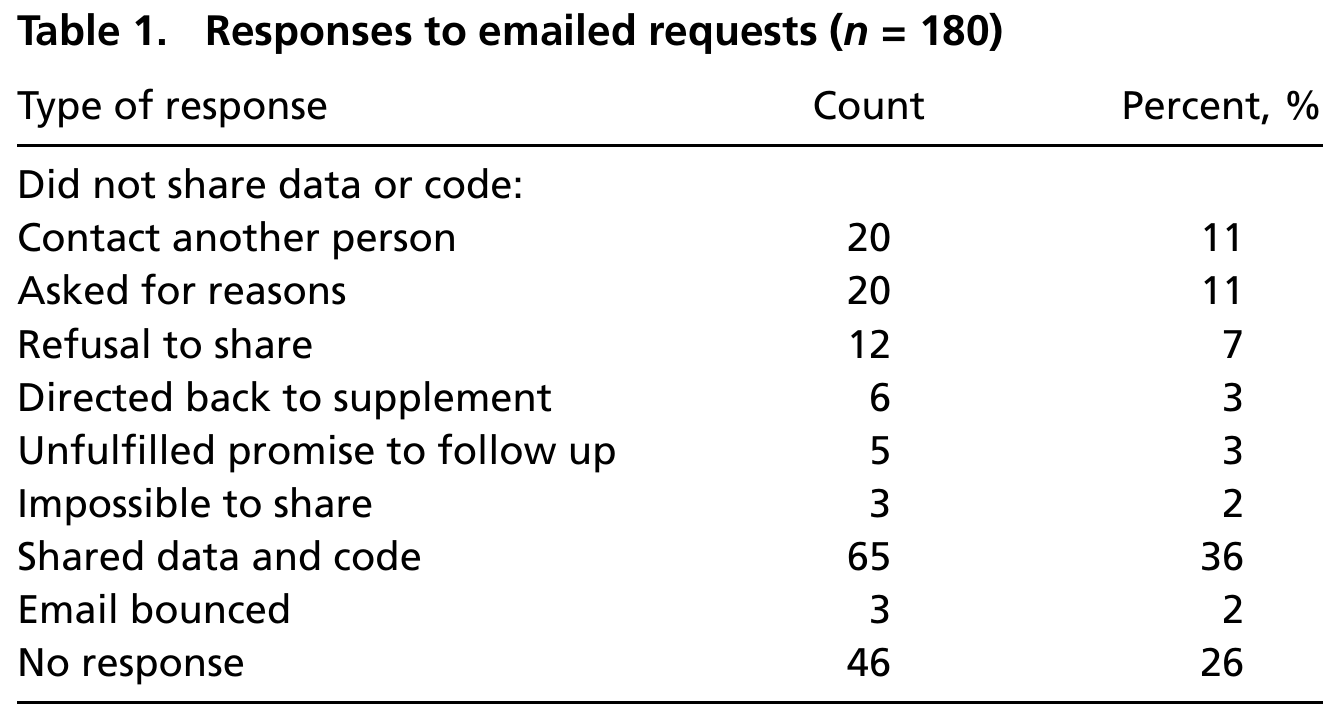
\includegraphics[width=0.9\textwidth]{%
      img/stodden2018_table1.png} %
  \end{figure}

  \vspace{0.1cm}
  
  \begin{center}
    $\Rightarrow$ Code \& data could be retrieved for 91 out of 206 studies.    
  \end{center}

  \source{\cite{Stodden2018}}
  
\end{frame}


